\begin{figure}[t]
    \centering
    \begin{subfigure}[b]{0.49\linewidth}
        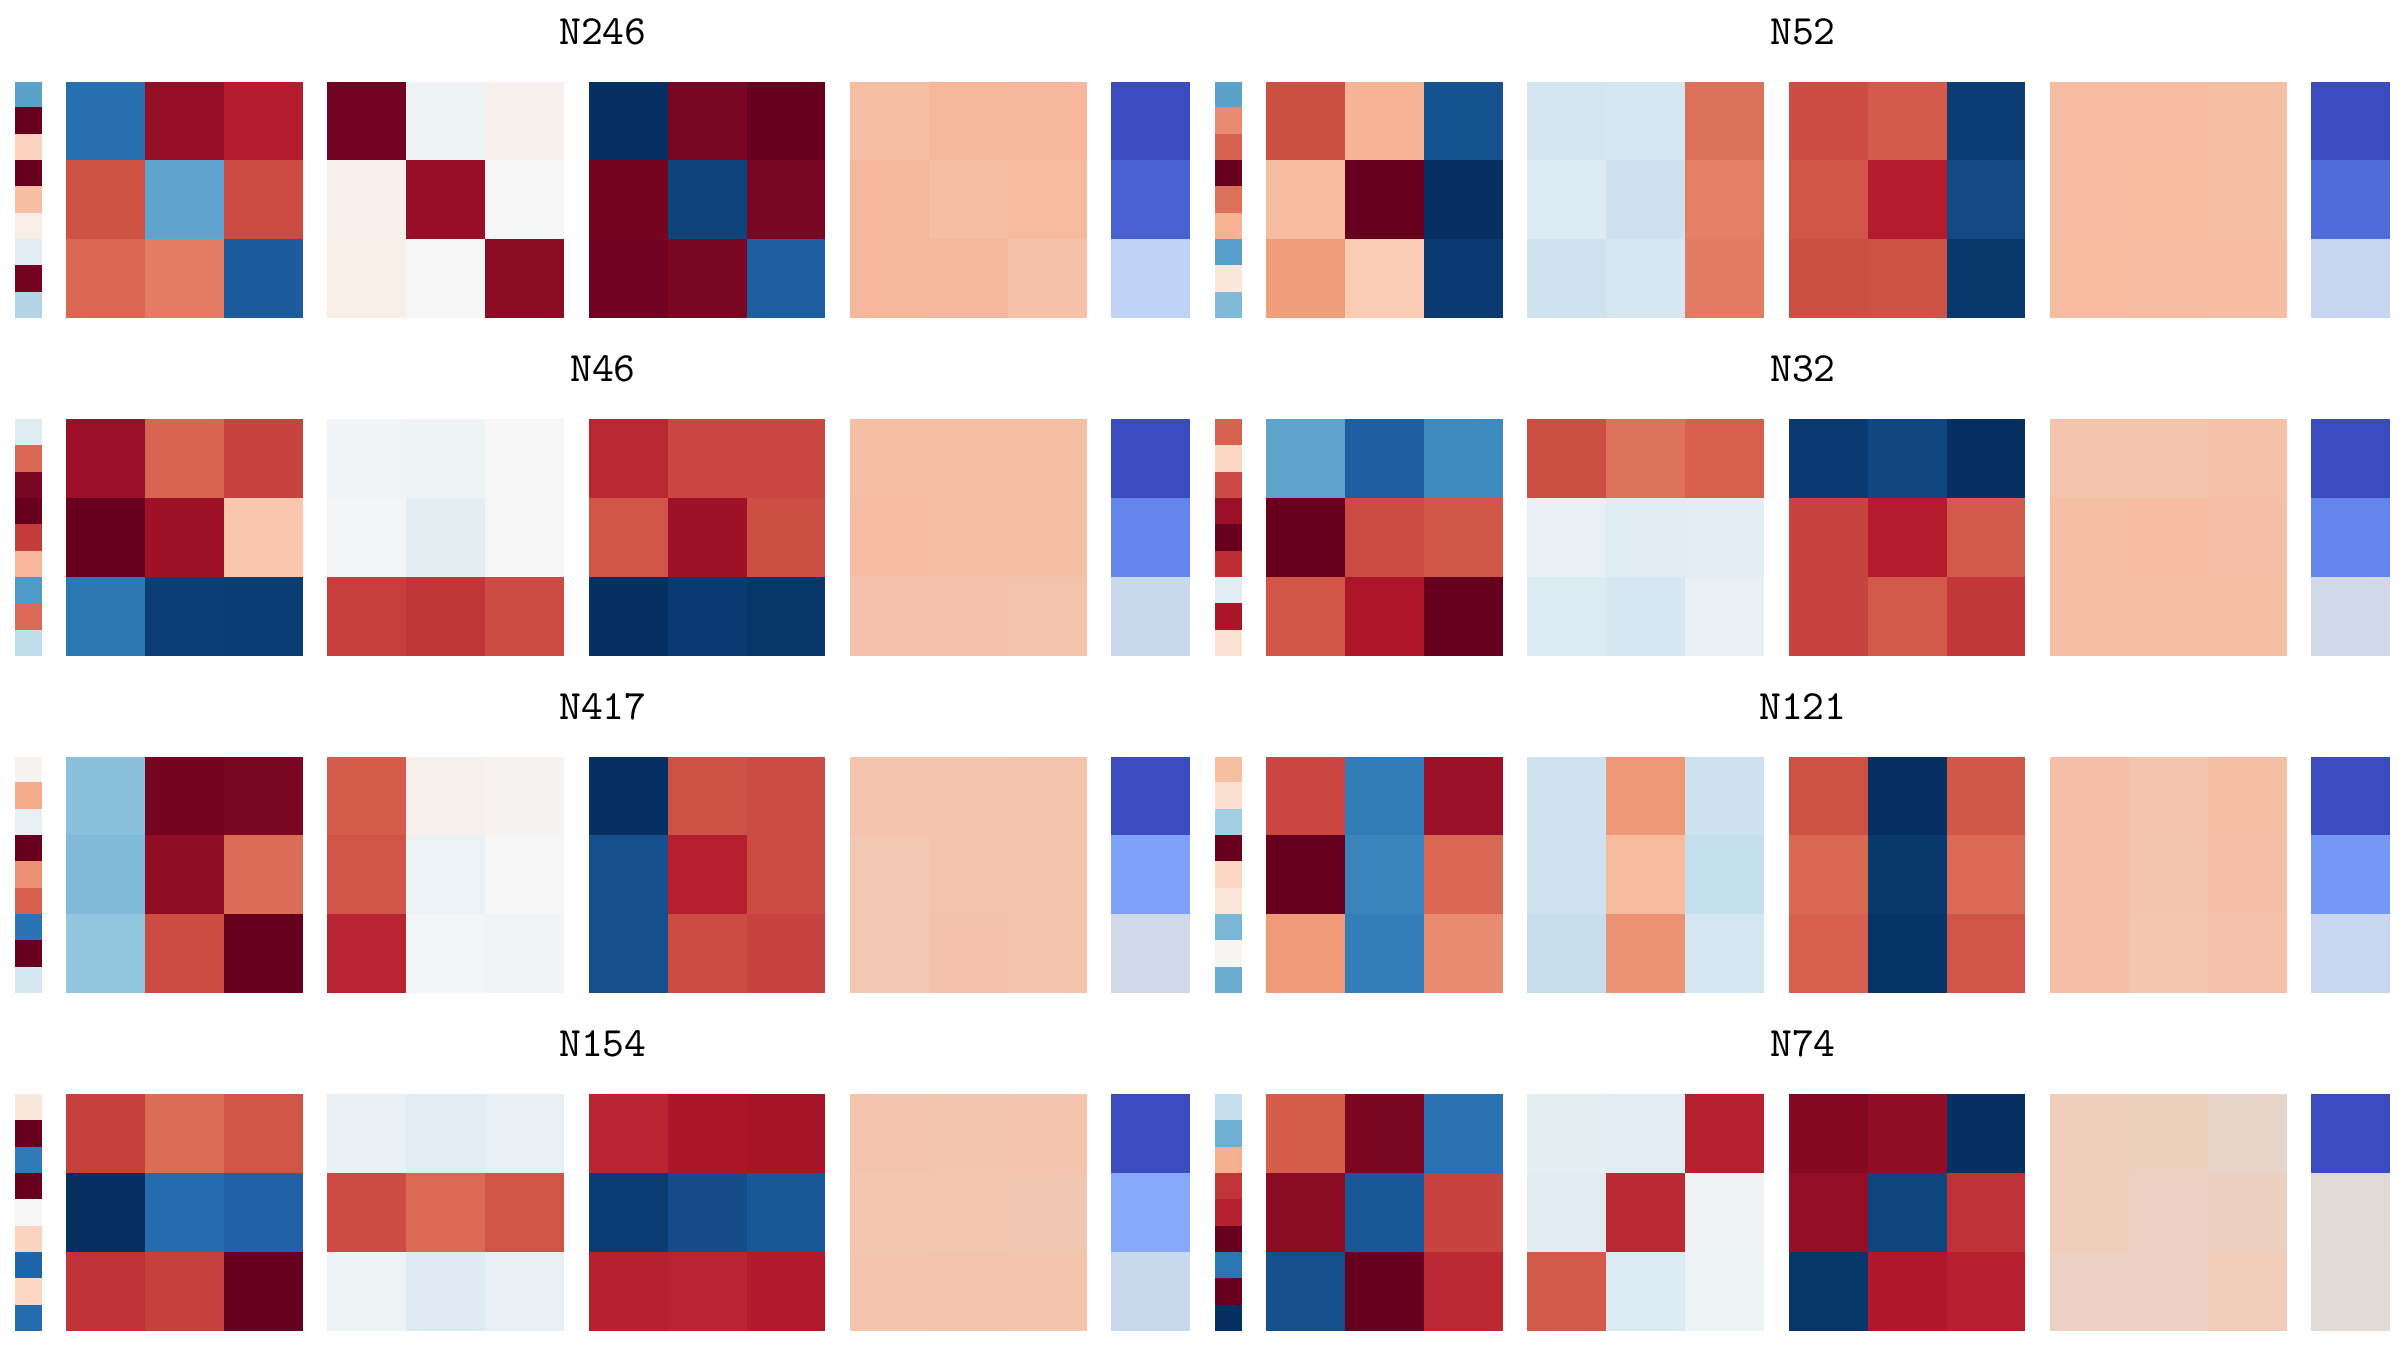
\includegraphics[width=\linewidth]{../out/figs/neuron_category_win_for_x.pdf}
        \caption{Identify wins for \texttt{X}.}
        \label{fig:neurons-x-win}
    \end{subfigure}%
    \hfill
    \begin{subfigure}[b]{0.49\linewidth}
        \includegraphics[width=\linewidth]{../out/figs/neuron_category_win_for_o.pdf}
        \caption{Identify wins for \texttt{O}.}
        \label{fig:neurons-o-win}
    \end{subfigure}
    \begin{subfigure}[b]{0.49\linewidth}
        \includegraphics[width=\linewidth]{../out/figs/neuron_category_move_suppression_single.pdf}
        \caption{Suppress moves already played.}
        \label{fig:neurons-suppress-single}
    \end{subfigure}%
    \hfill
    \begin{subfigure}[b]{0.49\linewidth}
        \includegraphics[width=\linewidth]{../out/figs/neuron_category_anti_win.pdf}
        \caption{Avoid playing moves that lead to wins.}
        \label{fig:neurons-suppress-win}
    \end{subfigure}
    \begin{subfigure}[b]{0.49\linewidth}
        \includegraphics[width=\linewidth]{../out/figs/neuron_category_draw.pdf}
        \caption{Predict draws.}
    \end{subfigure}
    \caption{Categorisation of the top neurons of \ttgpt into the ``rules'' they implement.}
    \label{fig:neuron-categories}
\end{figure}